\section{One-at-a-time}\label{sec:ot_oat}
This section discusses the results of the \gls{OAT} sensitivity analysis 
as applied to Scenario 7. A subset of this analysis is presented 
in \cite{bachmann_sensitivity_2022}, but the analysis presented here has 
an expanded scope and updated methodology to address the non-consistent 
replacement of advanced reactors in the previously published work.
The results in this subsection focus on 
the relative change in each metric for each parameter varied, because 
of the large range of the metric values. To that end, Table 
\ref{tab:oat_values} reports the minimum, 
average, and maximum value for each metric.

\begin{table}[ht!]
    \centering
    \caption{Minimum, average, and maximum value of each metric caused 
    by the variation of each parameter.}
    \label{tab:oat_values}
    \begin{tabular}{llrrrl}       
        \hline 
        Parameter &     Metric &      Minimum &      Average &      Maximum & Units\\
        \hline
        Transition Start &  Fuel Mass & 2.832e+07 & 3.001e+07 & 3.086e+07 & kg \\
                         & HALEU Mass & 2.777e+07 & 2.931e+07 & 3.005e+07 & kg\\ 
                         &  Total SWU & 9.727e+08 & 1.036e+09 & 1.068e+09 & kg-SWU\\ 
                         & HALEU SWU & 9.690e+08 & 1.031e+09 & 1.062e+09 & kg-SWU\\
                         &        UNF & 2.600e+07 & 2.744e+07 & 2.813e+07 & kg\\  
                         & HALEU Feed & 8.406e+08 & 8.936e+08 & 9.204e+08 & kg\\\hline
        LWR Lifetimes &  Fuel Mass & 2.226e+07 & 2.574e+07 & 2.934e+07 & kg\\
                      & HALEU Mass & 2.186e+07 & 2.528e+07 & 2.885e+07 & kg\\
                      &  Total SWU & 7.780e+08 & 8.973e+08 & 1.021e+09 & kg-SWU\\
                      &  HALEU SWU & 7.753e+08 & 8.941e+08 & 1.018e+09 & kg-SWU\\
                      &        UNF & 1.956e+07 & 2.305e+07 & 2.669e+07 & kg\\
                      & HALEU Feed & 6.716e+08 & 7.746e+08 & 8.820e+08 & kg\\\hline 
        Xe-100 Build Share &  Fuel Mass & 8.230e+07 & 1.130e+08 & 1.471e+08 & kg\\
                           & HALEU Mass & 2.827e+06 & 1.078e+07 & 1.804e+07 & kg\\
                           &  Total SWU & 1.083e+09 & 1.090e+09 & 1.102e+09 & kg-SWU\\
                           &  HALEU SWU & 1.275e+08 & 3.999e+08 & 6.501e+08 & kg-SWU\\
                           &        UNF & 7.511e+07 & 1.032e+08 & 1.344e+08 & kg\\
                           & HALEU Feed & 1.081e+08 & 3.448e+08 & 5.622e+08 & kg\\\hline 
        MMR Build Share &  Fuel Mass & 3.702e+07 & 4.918e+07 & 6.134e+07 & kg\\
                        & HALEU Mass & 2.670e+07 & 3.852e+07 & 5.039e+07 & kg\\
                        &  Total SWU & 9.901e+08 & 1.600e+09 & 2.212e+09 & kg-SWU\\
                        &  HALEU SWU & 9.205e+08 & 1.528e+09 & 2.138e+09 & kg-SWU\\
                        &        UNF & 3.440e+07 & 4.066e+07 & 4.689e+07 & kg\\
                        & HALEU Feed & 7.995e+08 & 1.310e+09 & 1.822e+09 & kg\\\hline 
        VOYGR Build Share &  Fuel Mass & 3.045e+07 & 6.436e+07 & 9.510e+07 & kg\\
                          & HALEU Mass & 1.516e+07 & 2.233e+07 & 3.045e+07 & kg\\
                          &  Total SWU & 1.077e+09 & 1.082e+09 & 1.092e+09 & kg-SWU\\
                          &  HALEU SWU & 5.528e+08 & 7.988e+08 & 1.080e+09 & kg-SWU\\
                          &        UNF & 2.765e+07 & 5.870e+07 & 8.679e+07 & kg\\
                          & HALEU Feed & 4.775e+08 & 6.913e+08 & 9.353e+08 & kg\\\hline 
        Xe-100 Burnup &  Fuel Mass & 2.761e+07 & 5.888e+07 & 1.591e+08 & kg\\
                      & HALEU Mass & 2.681e+07 & 5.809e+07 & 1.583e+08 & kg\\
                      &  Total SWU & 9.559e+08 & 2.034e+09 & 5.489e+09 & kg-SWU\\
                      &  HALEU SWU & 9.505e+08 & 2.029e+09 & 5.484e+09 & kg-SWU\\
                      &        UNF & 2.486e+07 & 5.614e+07 & 1.564e+08 & kg\\
                      & HALEU Feed & 8.233e+08 & 1.760e+09 & 4.761e+09 & kg\\\hline 
        MMR Burnup &  Fuel Mass & 3.065e+07 & 3.124e+07 & 3.293e+07 & kg\\
                   & HALEU Mass & 2.986e+07 & 3.045e+07 & 3.214e+07 & kg\\
                   &  Total SWU & 1.059e+09 & 1.085e+09 & 1.162e+09 & kg-SWU\\
                   &  HALEU SWU & 1.054e+09 & 1.080e+09 & 1.156e+09 & kg-SWU\\
                   &        UNF & 2.791e+07 & 2.850e+07 & 3.019e+07 & kg\\
                   & HALEU Feed & 9.128e+08 & 9.354e+08 & 1.000e+9 & kg\\
        \hline
    \end{tabular}
\end{table}


\subsection{Transition start time}
Delays in the transition start time generally decrease all of the output 
metrics, as shown in Figure \ref{fig:ts_scenario7}. This result matches 
expectations, because if the advanced reactors are deployed for less time, 
then they require fewer resources. However, there are some oscillations in 
the output metrics between individual time steps. For example, a transition 
start time of October 2029 increases the fuel mass and \gls{UNF} mass 
relative to July 2029, the start time previous. This increase results 
from changes in the number 
of each advanced reactor deployed, because of differences in the gap 
between energy produced and energy demand that must initially be filled when 
advanced reactors are deployed. By waiting until October 2029, more VOYGRs 
are deployed than when the transition starts in July 2029. As discussed in 
Chapter \ref{ch:once_through_results}, the VOYGR needs a larger fuel mass, 
and thus discharges more \gls{UNF} than the Xe-100 and \gls{MMR}. Therefore, 
these two metrics increase for this particular transition start time. 

\begin{figure}[h!]
    \centering
    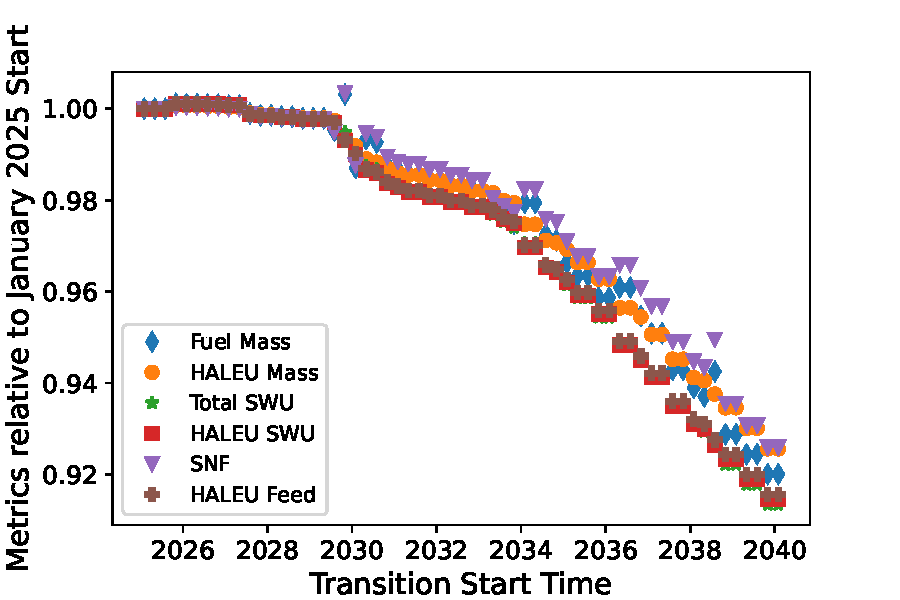
\includegraphics[scale=0.8]{ts.pdf}
    \caption{Change in each metric as a function of transition start 
    time, relative to a transition start in January 2025.}
    \label{fig:ts_scenario7}
\end{figure}

One of the disadvantages in delaying the transition start time is the 
increasing gap between energy supplied and energy demand as the transition 
start time is delayed. All of these scenarios have a constant demand 
of 87.20 GWe-yr beginning in January 2025. By delaying the transition start 
time to after September 2025 (the observed initial deployment time of advanced 
reactors in Section \ref{sec:nogrowth_reactors}), there is a difference
between the energy supplied and the energy demand. The largest gap observed 
is 36.7
GWe-yr, when reactors are deployed starting in January 2040. Therefore, 
delaying the transition start time is not an ideal method of 
potentially reducing materials to support advanced reactors. 

\subsection{LWR lifetimes}
The next metric varied is the percent of the \glspl{LWR} that operate for 
80 years, reflecting the effect license extensions in the \gls{LWR} fleet. 
Figure \ref{fig:lwr_scenario7} shows that the percent of the \gls{LWR} 
fleet operating for 80 years increases, all of the metrics decrease. 
All of the metrics decrease 
linearly and by a similar magnitude, with some variation because 
of changes in the number of each advanced reactor deployed, as discussed 
in Chapter \ref{ch:once_through_results}. The \gls{UNF} mass decreases 
more than the other metrics across 
this parameter space, ranging between 19.5-26.7 MTU.

\begin{figure}[h!]
    \centering
    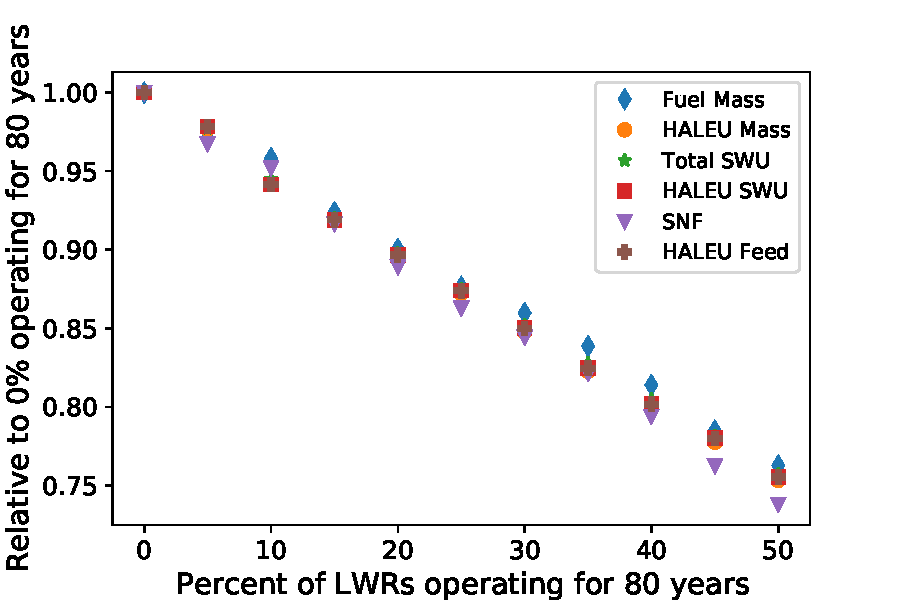
\includegraphics[scale=0.8]{lwr.pdf}
    \caption{Change in each metric as a function of percent of LWR fleet  
    operating for 80 years, relative to 0\%.}
    \label{fig:lwr_scenario7}
\end{figure}

Across this parameter space, the metrics decrease by a greater fraction than 
when varying the transition start time. The increased impact on the metrics 
is partly because of a small modeling change. When varying the transition 
start time, the \glspl{LWR} are assumed to have the same lifetime as the 
ones used in the transition analysis. Almost all of these lifetimes are  
60 years but there are a select few (such as Watts Bar Unit 2) that 
are currently licensed for 40 years. A simplifying assumption for 
modeling the effects of extending the \gls{LWR} lifetimes is that 
they operate for either 60 or 80 years, giving those select few reactors 
an artificial lifetime extension from 40 to 60 years, compared with the previous analysis. 
This modeling difference does not have a large impact on the results as 
evidenced by the maximum \gls{HALEU} mass when varying the \gls{LWR} lifetimes 
being only 4.9\% lower than the maximum \gls{HALEU} mass when varying the 
transition start time. Therefore, we can attribute most of the change in
the metrics to the 
change in the \gls{LWR} lifetimes and not the artificial increase in 
lifetimes from 40 to 60 years. Additionally, extending the \gls{LWR}
lifetimes inherently delays the start time of the transition, or at 
least decreases the speed of the transition, because the \glspl{LWR} 
are sufficient to meet the energy demand for a longer period of time.
In addition to causing greater change in the metrics, the energy demand 
is always met when varying the \gls{LWR} lifetimes, which suggests that 
extending the lifetimes of the \glspl{LWR} is a preferable parameter to vary 
if one wishes to decrease material requirements of this transition. 

\subsection{Xe-100 build share}
Figure \ref{fig:xe100_scenario7} shows that as the Xe-100 build share increases, 
the \gls{HALEU}-related metrics 
increase while the total \gls{UNF} and total fuel mass decrease and the 
total \gls{SWU} capacity stays relatively constant. Figure \ref{fig:xe100_s7_combined_reactors} 
shows that as the Xe-100 build share 
increases, the number of \glspl{MMR} is relatively constant and the number of 
VOYGRs decreases. These results show that as the Xe-100 build share 
increases, the Xe-100s are primarily replacing power that is supplied by 
the VOYGRs, instead of a portion of both of the other advanced reactors.
This replacement of VOYGRs is because of the deployment scheme used in this
work, as the VOYGR has the largest power output between the VOYGR and 
\gls{MMR}. Therefore, VOYGR deployment is maximized when the Xe-100 
build share is 0\%. This effect of the deployment scheme indicates that 
varying this parameter highlights trade-offs between the Xe-100 and 
VOYGR reactors.

\begin{figure}[h!]
    \centering
    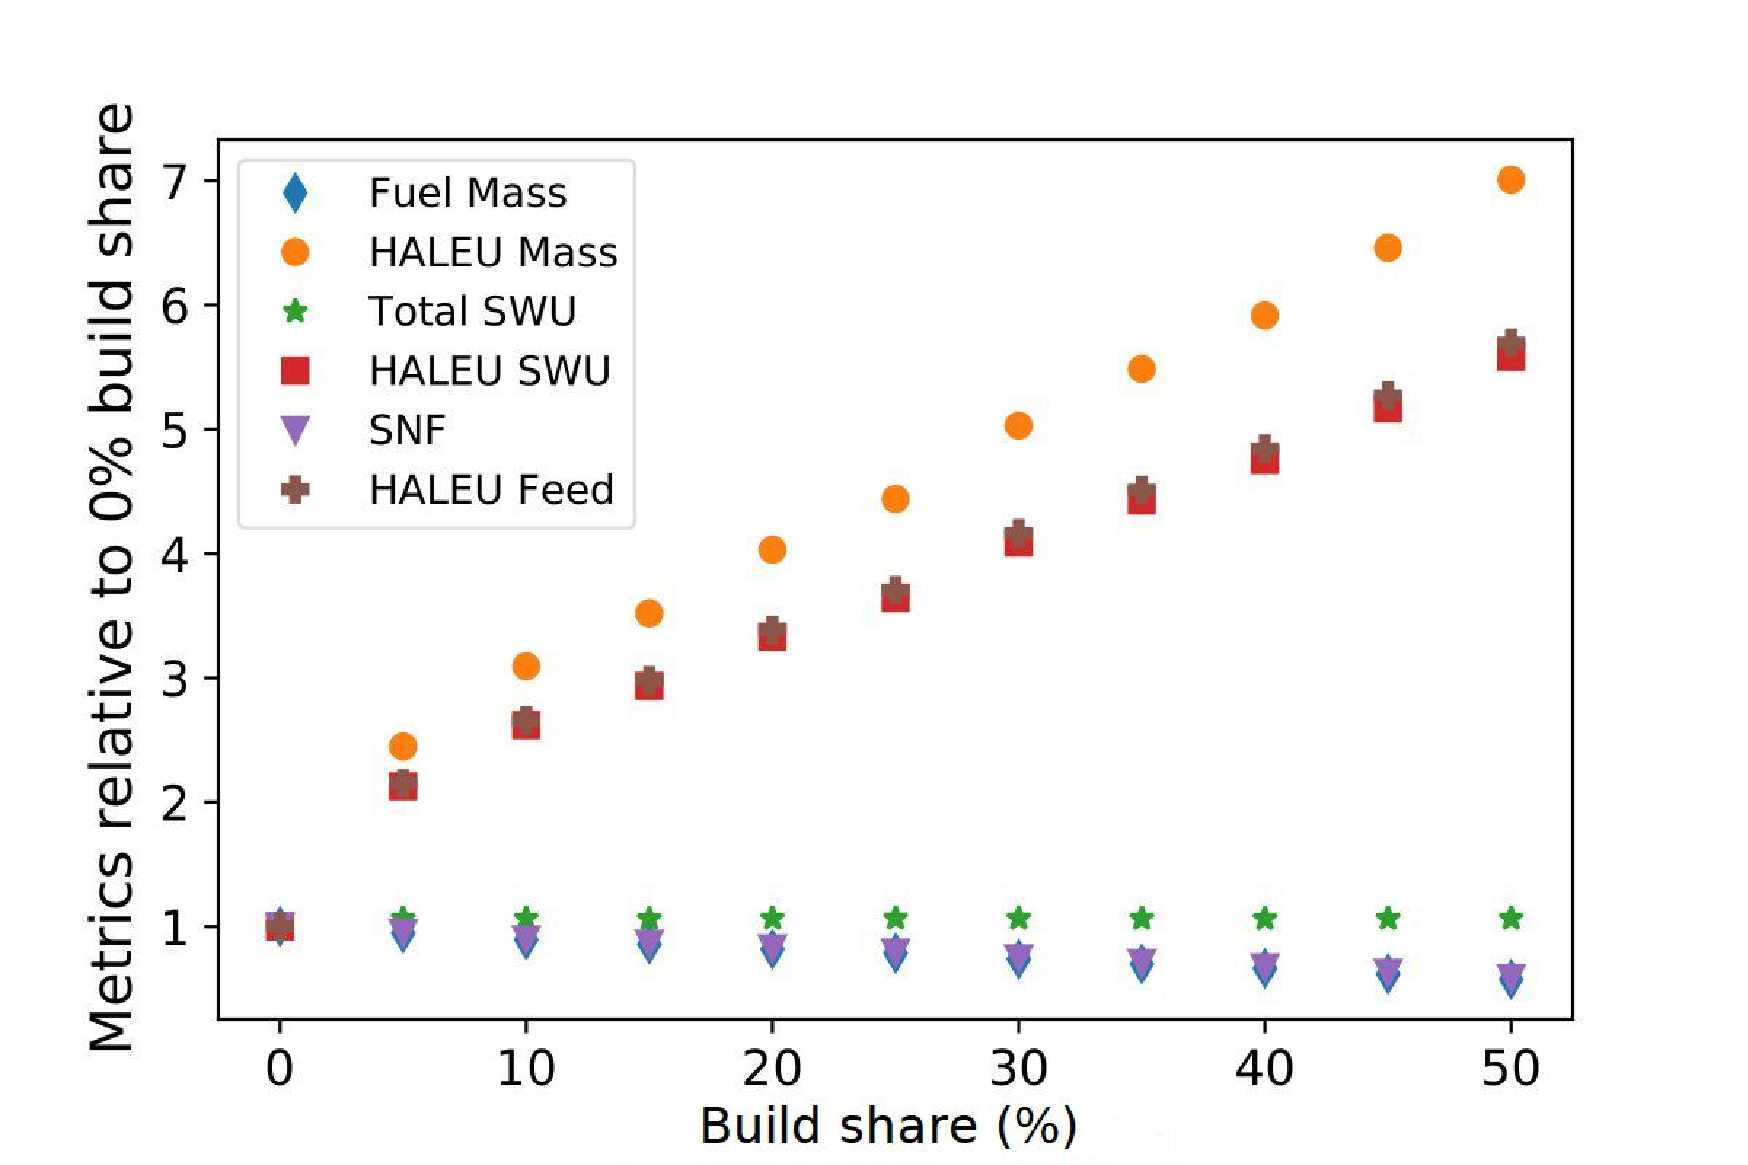
\includegraphics[scale=0.45]{xe100.pdf}
    \caption{Change in each metric as a function of Xe-100 build share, 
    relative to a build share of 0\%.}
    \label{fig:xe100_scenario7}
\end{figure}

\begin{figure}[h!]
    \centering
    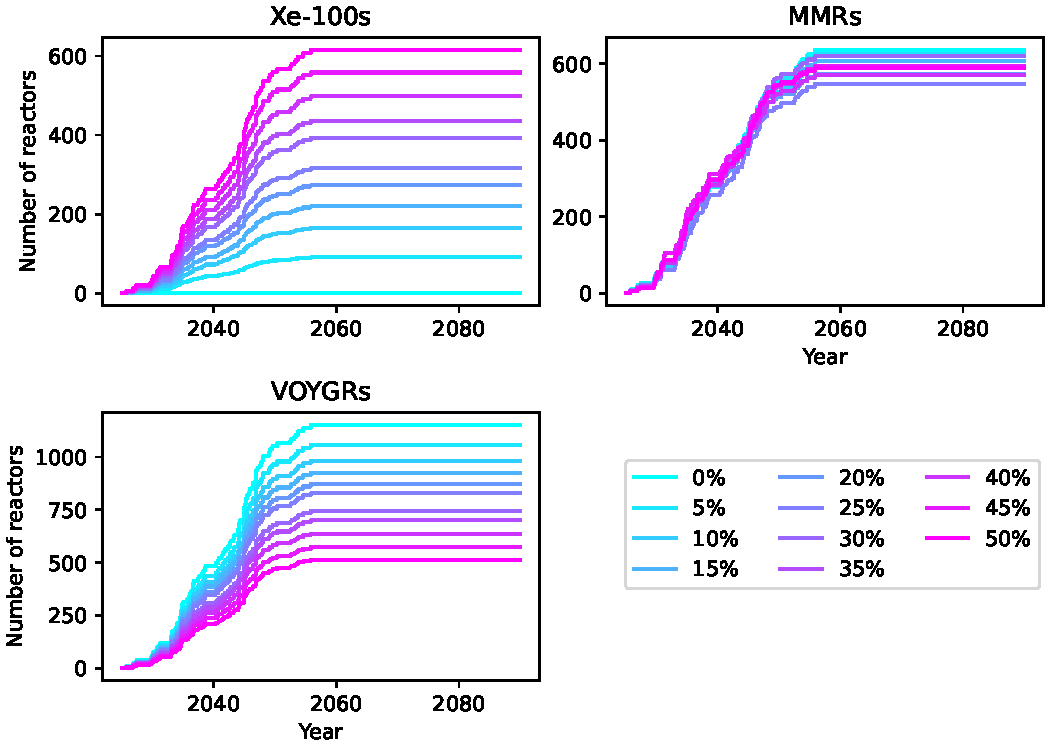
\includegraphics[scale=0.7]{xe100_combined_reactors.pdf}
    \caption{Number of Xe-100s (top left), MMRs (top right), and VOYGRs
    (bottom left) as a function of Xe-100 build share.}
    \label{fig:xe100_s7_combined_reactors}
\end{figure}

The \gls{HALEU}-related metrics increase with Xe-100 build share because more of 
the demand is met through advanced reactors requiring \gls{HALEU}. The total 
fuel mass and \gls{UNF} mass decrease because the 
Xe-100 requires less fuel per unit time and energy than the VOYGR, as discussed 
in Chapter \ref{ch:once_through_results}. The total \gls{SWU} capacity required 
is relatively constant, decreasing between 0.3-1.7\% compared to the \gls{SWU} capacity 
required for a 0\% Xe-100 build share. This stagnant behavior of the total 
\gls{SWU} capacity is consistent with the similar \gls{SWU} capacity required 
by Scenarios 3-7 in Section \ref{sec:nogrowth_swu}, when either the Xe-100 or 
VOYGR are primarily deployed. These results highlight the trade-off between the
\gls{HALEU}-related metrics and the total fuel mass and \gls{UNF} mass in deploying 
the Xe-100 versus the VOYGR. Both reactors require similar \gls{SWU} capacities 
but because of the different product assays required, the cascade configuration 
will vary. The \gls{HALEU}-related metrics increase up to 638\% of the 
mass required 
for a 0\% Xe-100 build share. The total fuel mass and \gls{UNF} mass decrease 
to up to 44.11\% of the mass required for 1 0\% Xe-100 build share. 

\subsection{MMR build share}
All of the metrics increase with increasing \gls{MMR} share, as shown 
in Figure \ref{fig:mmr_scenario7}. As the \gls{MMR} build share 
increases, the total \gls{SWU}, \gls{HALEU} \gls{SWU}, 
and \gls{HALEU} feed have the greatest relative increase because more of the 
advanced reactor fleet uses the highest enrichment level of the three 
advanced reactors. The \gls{HALEU} mass 
increases with the \gls{MMR} build share \glspl{MMR} replace Xe-100s
as the build share increases, shown in  
Figure \ref{fig:mmr_reactors_s7}.
The \gls{MMR} requires a greater fuel mass than the Xe-100, causing the increase 
in the \gls{HALEU} mass as \glspl{MMR} replace Xe-100s. 
The larger fuel mass required by the \gls{MMR}, compared 
with the Xe-100, compounds with the higher enrichment required by the \gls{MMR} 
to cause the greater relative increase in the total \gls{SWU}, \gls{HALEU} \gls{SWU}, 
and \gls{HALEU} feed. 

\begin{figure}[h!]
    \centering
    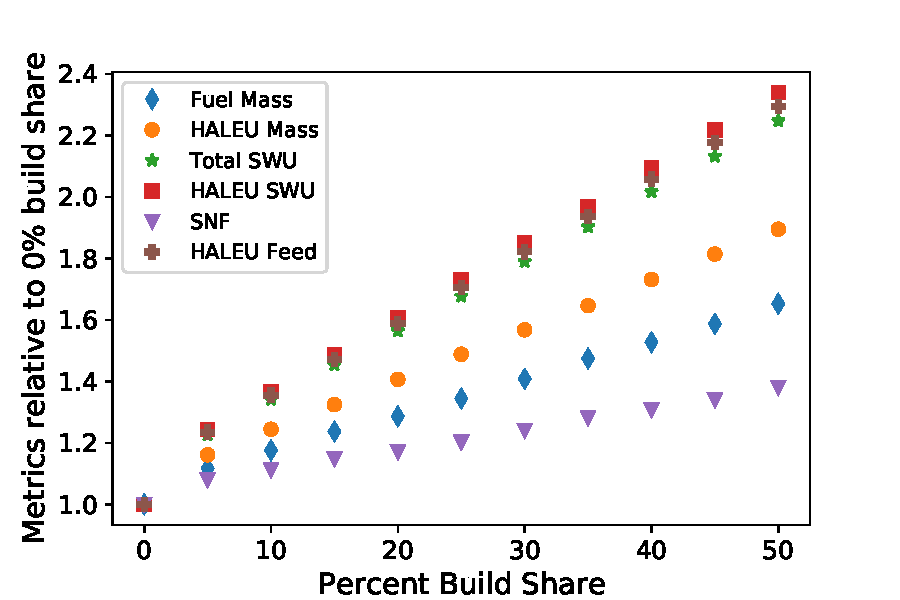
\includegraphics[scale=0.45]{mmr.pdf}
    \caption{Change in each metric as a function of MMR build share, 
    relative to a build share of 0\%.}
    \label{fig:mmr_scenario7}
\end{figure}


\begin{figure}[h!]
    \centering
    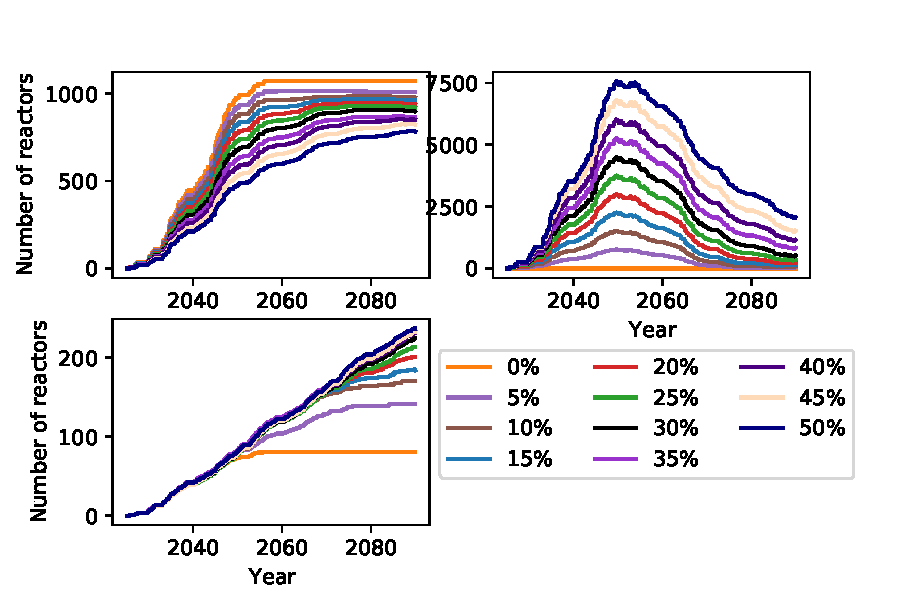
\includegraphics[scale=0.7]{mmr_combined_reactors.pdf}
    \caption{Number of Xe-100s (top left), MMRs (top right), and 
    VOYGRs (bottom left) deployed as a function of time and 
    MMR build share.}
    \label{fig:mmr_reactors_s7}
\end{figure}

The \gls{UNF} mass does not experience the same 
relative increase as the total fuel mass because any fuel that is still in a 
reactor core at the end of the simulation is not accounted for in the 
\gls{UNF} mass. Therefore, as the \gls{MMR} build share increases, more 
of the enriched uranium sent to reactors is still in a reactor core
at the end of the simulation because of the long cycle time of the 
\gls{MMR}. 
Based on the replacement of Xe-100s with \glspl{MMR} as the \gls{MMR} 
build share increases, these results highlight the effects of deploying the
\gls{MMR} over the Xe-100. 

\subsection{VOYGR build share}
Varying the VOYGR build share causes trends that are opposite 
to the effects observed from varying the Xe-100 build share. 
(Figure 
\ref{fig:voygr_scenario7}). The total fuel mass and \gls{UNF} mass 
increase, the \gls{HALEU}-related metrics decrease, and the total 
\gls{SWU} capacity remains relatively constant. This reversal 
of trends occurs because there is a replacement of Xe-100s with VOYGRs
with increasing build share (Figure \ref{fig:voygr_reactors_s7}), 
the opposite of what happens with an increasing Xe-100 build share. 

\begin{figure}[h!]
    \centering
    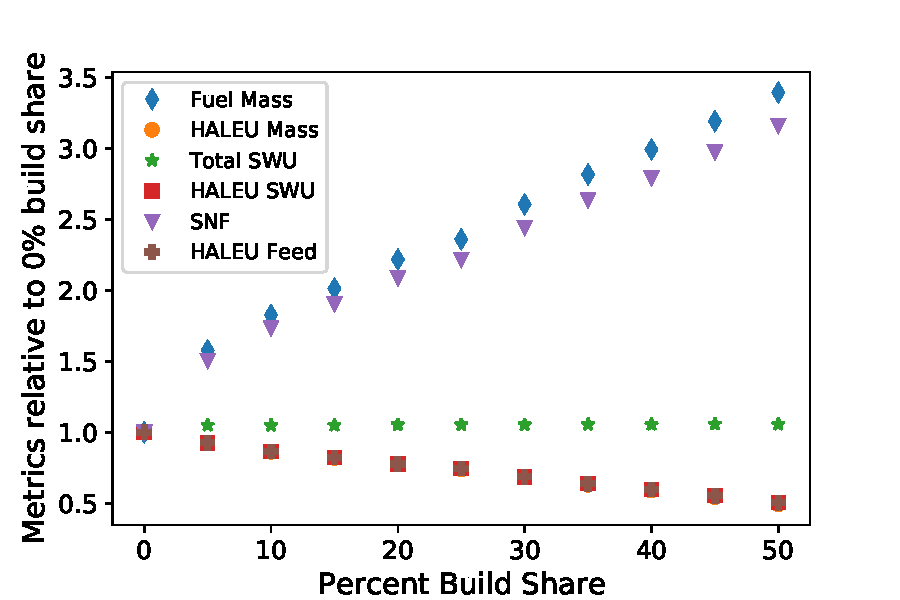
\includegraphics[scale=0.45]{voygr.pdf}
    \caption{Change in each metric as a function of VOYGR build share, 
    relative to a build share of 0\%.}
    \label{fig:voygr_scenario7}
\end{figure}

\begin{figure}[h!]
    \centering
    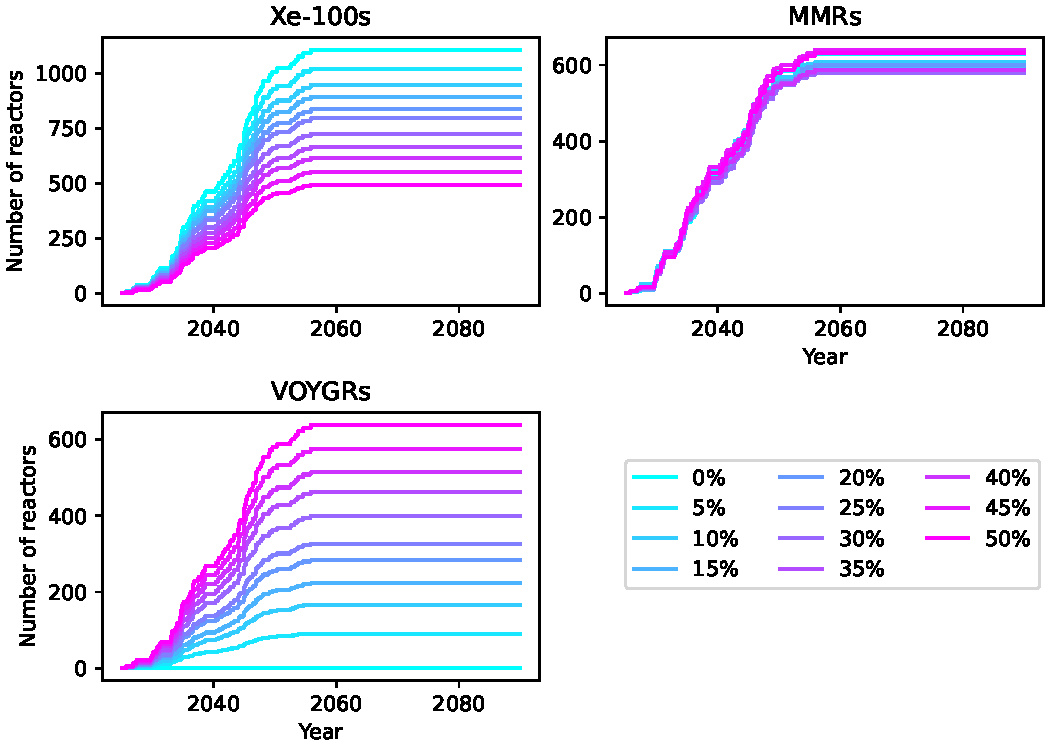
\includegraphics[scale=0.7]{voygr_combined_reactors.pdf}
    \caption{Number of Xe-100s (top left), MMRs (top right), and 
    VOYGRs (bottom left) deployed as a function of time and 
    VOYGR build share.}
    \label{fig:voygr_reactors_s7}
\end{figure}

The total \gls{SWU} capacity required varies between 99.6\%-101.2\% of the 
\gls{SWU} capacity needed for a 0\% VOYGR build share, a range of 1.077$\times 10^9$
- 1.092$\times 10^9$ kg-SWU (Table \ref{tab:oat_values}). The total fuel mass 
and \gls{UNF} mass increase 
up to 313.9\% of the mass required for a 0\% VOYGR build share, and the 
\gls{HALEU}-related metrics decrease to 49.77\% of the mass required 
for a 0\% VOYGR build share. The \gls{UNF} and total fuel masses increase 
because the VOYGR requires more fuel than the Xe-100, largely stemming from 
the difference in discharge burnup of these two reactors. The \gls{HALEU}-related 
metrics all decrease because the VOYGR does not require \gls{HALEU}. As the 
VOYGR build share increases a smaller portion of the advanced reactor fleet 
requires \gls{HALEU}. While the trends from varying the VOYGR build share 
mirrors the trends from varying the Xe-100 build share, the magnitude of the 
changes are not the same because these 
parameter variations cover adjacent but not overlapping design spaces. 

\subsection{Xe-100 burnup}
When varying the burnup of fuel discharged from Xe-100s, the metrics decrease 
as the burnup increases (Figure \ref{fig:xe100_bu_s7}). The material 
requirements decrease with increasing burnup because there are more 
batches of fuel or the fuel spends more time in the core.  
Therefore, the Xe-100s in the simulation are receiving 
less fuel at each refueling or receiving fuel less often as the burnup increases. 
Varying the burnup of the Xe-100 has a large impact on the metrics; the Xe-100 
reaching a burnup of 28 MWd/kg burnup requires up to fives times 
the material requirements compared with the designed burnup of 168 MWd/kgU.
When varying this parameter, most of the energy is met through deploying 
Xe-100s, so their fuel needs drive the total fuel cycle needs. 
Therefore, changes to the Xe-100 refueling is 
magnified because of their large deployment. 

\begin{figure}[h!]
    \centering
    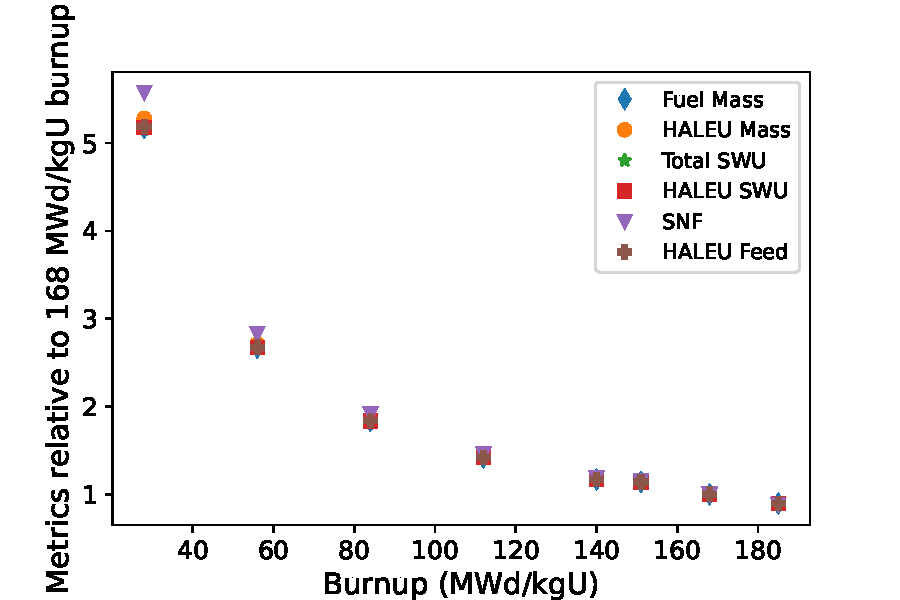
\includegraphics[scale=0.8]{xe100_bu.pdf}
    \caption{Change in metrics from varying the burnup of fuel 
    discharged from Xe-100, relative to a burnup of 168 MWd/kgU.}
    \label{fig:xe100_bu_s7}
\end{figure}

\subsection{MMR burnup}
When varying the \gls{MMR} discharge burnup, all of the metrics decrease, similar 
to what was observed by varying the Xe-100 discharge burnup, as shown in 
Figure \ref{fig:mmr_bu_s7}. One difference in 
the trends observed between varying these two parameters is the magnitude of 
the relative changes. Varying the \gls{MMR} burnup has a smaller relative effect 
on the metrics than varying the Xe-100 burnup because the \glspl{MMR}
meet a much smaller portion of the energy demand than the Xe-100s.
Therefore the impact on the cumulative metrics 
(what is reported here) is smaller. Another difference is that the total 
\gls{SWU}, \gls{HALEU} \gls{SWU}, and \gls{HALEU} feed increase the most 
when the \gls{MMR} burnup is low, compared with the \gls{UNF} having the 
greatest relative increase with the Xe-100 burnup is low. The difference 
in the relative change in \gls{UNF} is a result of the long cycle 
time of the \gls{MMR} and the results not accounting for 
\gls{UNF} still in a reactor at the end of the simulation, 
as previously discussed. 

\begin{figure}[h!]
    \centering
    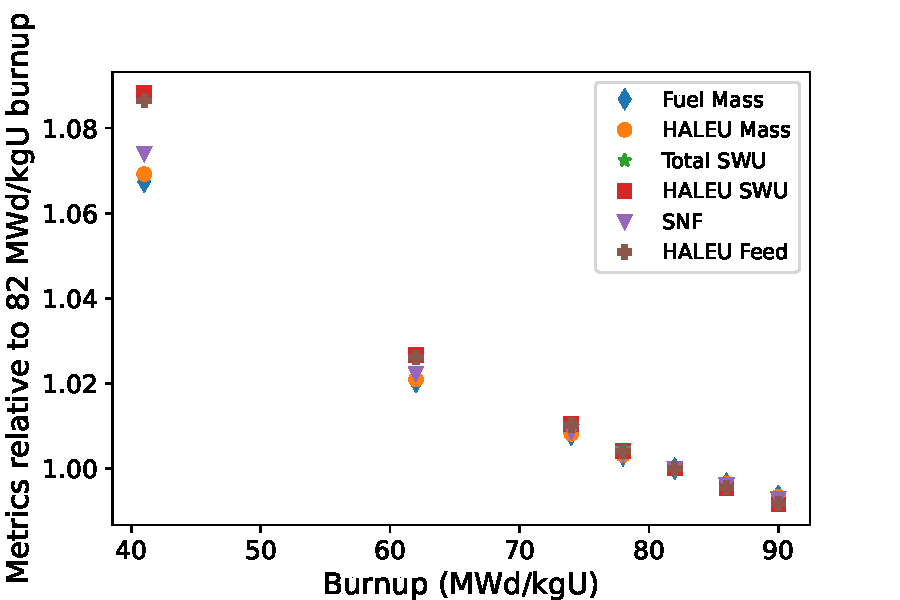
\includegraphics[scale=0.8]{mmr_bu.pdf}
    \caption{Change in metrics from varying the burnup of fuel 
    discharged from the MMR, relative to a burnup of 82 MWd/kgU.}
    \label{fig:mmr_bu_s7}
\end{figure}

\subsection{Burnup variations with a common build share}
To better investigate the effect of varying the discharge burnup of the Xe-100 
and \gls{MMR} without the influence of the deployment scheme preferentially
deploying Xe-100s, we repeated each set of analysis using a constant 20\% 
build share for both the Xe-100 and \gls{MMR} (VOYGRs meet the remaining 60\%). 
Using a constant build share for 
both reactors means that they each will supply the same fraction of the energy demand.
However, because of the different power output for each reactor a constant build 
share does not mean that the same number of each reactor is built. 

Figure \ref{fig:bu_constant} shows the relative change in each metric as a result 
of varying the \gls{MMR} (Figure \ref{fig:mmr_bu_constant}) and Xe-100 
(Figure \ref{fig:xe100_bu_constant}) discharge burnup with the constant build 
share. Changing the \gls{MMR} burnup has a greater impact with the specified 20\% 
build share than when the build share was not specified. This change is because 
more \glspl{MMR} are deployed with a 20\% build share than when the build share is 
not specified. Conversely, the Xe-100 burnup has a smaller impact on the metrics 
with a 20\% build share than when a build share isn't specified because fewer 
Xe-100s are deployed. 

\begin{figure}[h!]
    \centering
    \begin{subfigure}{0.48\textwidth}
        \centering
        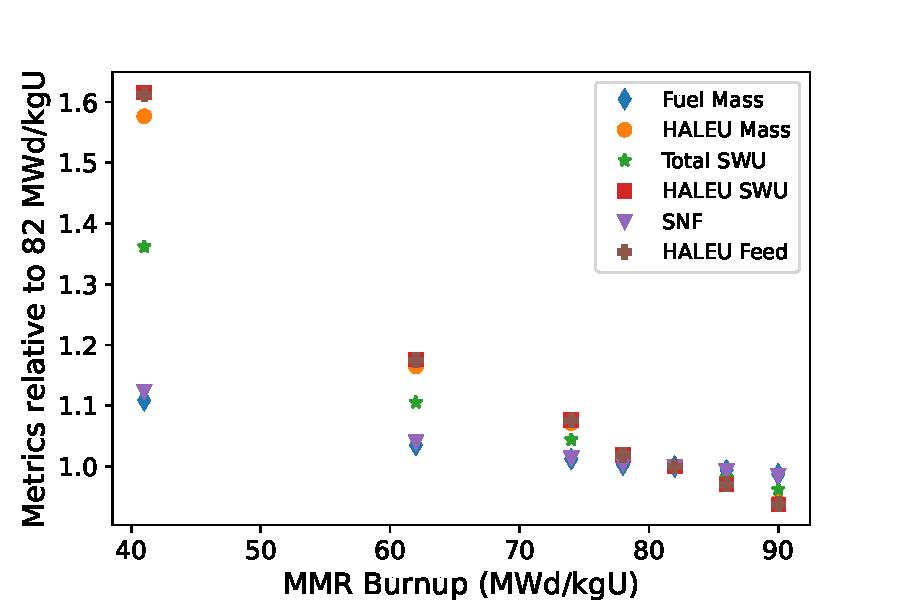
\includegraphics[width=\textwidth]{mmr_bu_constant.pdf}
        \caption{Change in metrics when varying the MMR discharge burnup.}
        \label{fig:mmr_bu_constant}
    \end{subfigure}
    \hfill
    \begin{subfigure}{0.48\textwidth}
        \centering
        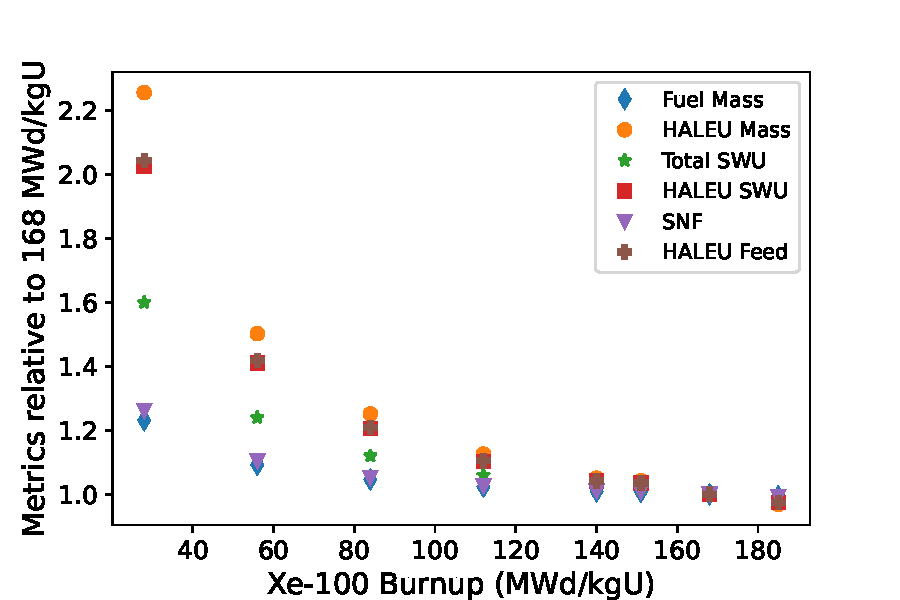
\includegraphics[width=\textwidth]{xe100_bu_constant.pdf}
        \caption{Change in metrics when varying the Xe-100 discharge burnup.}
        \label{fig:xe100_bu_constant}
    \end{subfigure}
    \caption{Relative changes in the metrics caused by changes in the discharge 
    burnup of the HALEU-fueled advanced reactors, assuming a constant 
    20\% build share for the Xe-100 and MMR.}
    \label{fig:bu_constant}
\end{figure}

By applying a constant build share, variations in these parameters lead to 
more variation in the effect on the metrics than when a build share was not 
specified. In these scenarios, varying the discharge burnup of either reactor 
leads to the greatest impact on the \gls{HALEU}-related metrics while the  
total fuel mass and \gls{UNF} mass are affected the least. 
The \gls{HALEU}-related metrics are affected the most because most of the 
energy demand is met through VOYGRs, which do not require \gls{HALEU}. 
Small changes in the each of the \gls{HALEU}-related metrics led to larger 
relative changes because these two reactors drive the effects on the 
\gls{HALEU}-related metrics. Conversely, the total fuel mass and \gls{UNF} 
masses are affected less by changes in these parameters because the fuel 
and \gls{UNF} for the VOYGRs are constant and the Xe-100 and \gls{MMR} 
have less of an impact on these two metrics. 